\documentclass[11pt]{article}

%%%%%%%%%%%%%%%%%%%%%%%%%%%%%%%%%%%%%%%%
% PACKAGES
%%%%%%%%%%%%%%%%%%%%%%%%%%%%%%%%%%%%%%%%
\usepackage[margin=1in]{geometry}
\usepackage{amsmath,amsfonts,amssymb}
\usepackage{xcolor}
\usepackage{graphicx}
\usepackage{tikz}
\usetikzlibrary{arrows.meta, positioning, shapes.geometric, calc}
\usepackage{hyperref}
\usepackage{enumitem}
\usepackage{longtable}
\usepackage{titlesec}
\usepackage{array}
\usepackage{booktabs}

%%%%%%%%%%%%%%%%%%%%%%%%%%%%%%%%%%%%%%%%
% COLOR SCHEME (black/blue/red)
%%%%%%%%%%%%%%%%%%%%%%%%%%%%%%%%%%%%%%%%
\definecolor{myblue}{RGB}{20,90,160}
\definecolor{myred}{RGB}{180,40,40}
\newcommand{\blue}[1]{\textcolor{myblue}{#1}}
\newcommand{\red}[1]{\textcolor{myred}{#1}}
\newcommand{\term}[1]{\textbf{\blue{#1}}}
\newcommand{\danger}[1]{\textbf{\red{#1}}}

\hypersetup{
  colorlinks=true,
  linkcolor=myblue,
  urlcolor=myblue,
  citecolor=myblue
}

%%%%%%%%%%%%%%%%%%%%%%%%%%%%%%%%%%%%%%%%
% SECTION STYLING
%%%%%%%%%%%%%%%%%%%%%%%%%%%%%%%%%%%%%%%%
\titleformat{\section}
{\large\bfseries\color{myblue}}
{\thesection}{1em}{}

\titleformat{\subsection}
{\bfseries\color{myblue}}
{\thesubsection}{1em}{}

%%%%%%%%%%%%%%%%%%%%%%%%%%%%%%%%%%%%%%%%
% MEMORY BOXES (same structure + scheme)
%%%%%%%%%%%%%%%%%%%%%%%%%%%%%%%%%%%%%%%%
\newenvironment{bluebox}
{\vspace{6pt}\noindent\begin{tikzpicture}
\node[
draw=myblue, line width=1pt,
rounded corners=6pt,
inner sep=8pt,
text width=\dimexpr\linewidth-20pt\relax
]\bgroup
\begin{minipage}{\dimexpr\linewidth-32pt\relax}
\blue{\textbf{Key Idea}}\par\vspace{4pt}}
{\end{minipage}\egroup;\end{tikzpicture}\vspace{6pt}}

\newenvironment{redbox}
{\vspace{6pt}\noindent\begin{tikzpicture}
\node[
draw=myred, line width=1pt,
rounded corners=6pt,
inner sep=8pt,
text width=\dimexpr\linewidth-20pt\relax
]\bgroup
\begin{minipage}{\dimexpr\linewidth-32pt\relax}
\red{\textbf{Important}}\par\vspace{4pt}}
{\end{minipage}\egroup;\end{tikzpicture}\vspace{6pt}}

%%%%%%%%%%%%%%%%%%%%%%%%%%%%%%%%%%%%%%%%
% QUICK FILL LINES
%%%%%%%%%%%%%%%%%%%%%%%%%%%%%%%%%%%%%%%%
\newcommand{\fillline}[1]{\noindent\textbf{#1}\ \underline{\hspace{11.2cm}}\par}
\newcommand{\fillpar}[1]{\noindent\textbf{#1}\par\vspace{0.25cm}\noindent\underline{\hspace{\linewidth}}\par\vspace{0.25cm}\underline{\hspace{\linewidth}}\par}
\newcommand{\ProjectHeader}[2]{
\section{#1}
\begin{bluebox}
\textbf{Stack:} #2
\end{bluebox}
}

%%%%%%%%%%%%%%%%%%%%%%%%%%%%%%%%%%%%%%%%
% DOC HEADER
%%%%%%%%%%%%%%%%%%%%%%%%%%%%%%%%%%%%%%%%
\title{\blue{Interview Project Notes (45-min Ready)}\\ \large Minimal talk-tracks + core concepts + expected questions}
\author{}
\date{}

\begin{document}
\maketitle

% ===========================
% CLEANED + ORGANIZED SECTION
% (spell/grammar fixed, redundancy trimmed, logic clarified)
% Colors used intentionally: BLUE = definitions/structure, RED = pitfalls/limits
% ===========================

\begin{bluebox}
    \textbf{Need-to-knows (Performance + Scaling Cheat Sheet)}
    \end{bluebox}
    
\textbf{CPU architecture:}
\begin{itemize}
\item A small number of cores, each with its own L1 cache and control logic attached.
\item L2/L3 caches sit outside / above the cores (shared at higher levels).
\end{itemize}

\textbf{GPU architecture:}
\begin{itemize}
\item Many cores (lots of parallel lanes).
\item L1 cache + shared memory close to execution units; L2 cache shared; DRAM = high bandwidth memory (HBM).
\item Optimized for moving data fast and doing lots of arithmetic per unit time.
\end{itemize}

    \begin{itemize}[leftmargin=1.2em]
    
    % ---------------------------
    % Roofline / Operational Intensity
    % ---------------------------
    \item \term{Operational Intensity (OI)} (a.k.a. arithmetic intensity):  
    \[
    \text{OI} \;=\; \frac{\text{FLOPs}}{\text{Bytes moved to/from memory}}
    \]
    \begin{bluebox}
    \textbf{Roofline intuition:} achievable performance is limited by either \blue{compute} or \blue{memory bandwidth}.
    \[
    \text{Perf} \;\le\; \min\Big(\text{Peak FLOPs/s},\; \text{OI} \times \text{Peak BW}\Big)
    \]
    \end{bluebox}
    
    \textbf{How to interpret:}
    \begin{itemize}
    \item \blue{Low OI} $\rightarrow$ \textbf{memory-bound} (limited by bandwidth).  
    Fixes: reuse data (tiling/fusion), reduce reads/writes, improve locality, mixed precision.
    \item \blue{High OI} $\rightarrow$ \textbf{compute-bound}.  
    Fixes: use vectorization/tensor cores, improve occupancy, reduce divergence, improve instruction mix.
    \end{itemize}
    
    \begin{center}
    \renewcommand{\arraystretch}{1.15}
    \begin{tabular}{|p{0.20\linewidth}|p{0.36\linewidth}|p{0.36\linewidth}|}
    \hline
    \textbf{Regime} & \textbf{What you see} & \textbf{What you do} \\
    \hline
    Compute-bound & high SM active, BW not maxed, kernels dominate runtime & increase tensor core use, fuse kernels, improve occupancy, reduce divergence \\
    \hline
    Memory-bound & BW near peak, moderate SM active, lots of stalls & tiling, shared memory/cache reuse, coalescing, fewer global reads/writes \\
    \hline
    I/O-bound & GPU idle, data loader maxed, disk/network busy & caching, preprocessing offline, parallel loading, faster storage/network \\
    \hline
    \end{tabular}
    \end{center}
    
    % ---------------------------
    % The big 3 bottlenecks (HPC)
    % ---------------------------
    \item \term{In HPC/AI infra, performance issues usually fall into 3 buckets:}
    
    \begin{enumerate}[leftmargin=1.2em]
    % ---- 1) Compute bound
    \item \blue{\textbf{Compute-bound}}
    \begin{itemize}
    \item \textbf{Signs:} GPU utilization is high (often 90--100\%), memory bandwidth is \textbf{not} maxed, kernels take most of runtime, pipeline is keeping up.
    \item \textbf{Tools:}
    \begin{itemize}
    \item \term{Nsight Compute (NCU):} \texttt{ncu --set full ./your\_app} \ \ (\textbf{INSERT complete}).
    \item \term{Nsight Systems (NSYS):} \texttt{nsys profile ./your\_app} \ \ (timeline + CPU/GPU overlap).
    \item \term{PyTorch Profiler:} \texttt{torch.profiler} for operator-level breakdown.
    \item \term{CPU:} \texttt{top}, \texttt{htop}.
    \item \term{Cluster:} Slurm job stats (e.g., \texttt{squeue}, \texttt{sstat}, \texttt{sacct}).
    \end{itemize}
    
    \item \textbf{Solutions (systems):} kernel fusion, better parallelism, vectorization (warps/TC), reduce divergence, tune block sizes/occupancy.
    \item \textbf{Solutions (ML):} mixed precision (FP16/BF16/INT8), quantization, pruning, and batch tuning (bigger batch $\rightarrow$ faster but more memory; smaller batch $\rightarrow$ slower but safer memory).
    \end{itemize}
    
    % ---- 2) Memory bound
    \item \blue{\textbf{Memory-bound}}
    \begin{itemize}
    \item \textbf{Signs:} GPU utilization is moderate, memory bandwidth is near peak, kernels stall on memory; profilers show memory bottlenecks (cache misses, uncoalesced access, large tensors moving around).
    \item \textbf{Where common:} CNNs and Transformers can be memory-heavy; runtime is often dominated by tensor movement.
    \item \textbf{Solutions:}
    \begin{itemize}
    \item \term{Coalescing:} make neighboring threads access neighboring memory (e.g., column-wise indexing like \texttt{col = baseCol + threadIdx.x}).
    \item \term{Reuse:} shared memory / cache tiles, blocking/tiling.
    \item \term{Reduce traffic:} avoid unnecessary copies, fuse ops, reduce precision.
    \item \term{ML tricks:} gradient checkpointing, activation recomputation, better batching.
    \end{itemize}
    \end{itemize}
    
    % ---- 3) I/O bound
    \item \blue{\textbf{I/O-bound}}
    \begin{itemize}
    \item \textbf{Signs:} GPU is idle waiting for data, disk/network activity is high, training pauses intermittently, CPU data loader is maxed.
    \item \textbf{Tools:} \texttt{iostat}, \texttt{iftop}/\texttt{nload} (network), \texttt{nvidia-smi} utilization drops, Slurm job stats.
    \item \textbf{Solutions:}
    \begin{itemize}
    \item dataset caching, preprocessing offline, parallel data loaders
    \item faster storage (SSD/NVMe), reduce contention
    \item distributed: InfiniBand/RDMA, dataset sharding, node-local caching/sharing
    \end{itemize}
    \end{itemize}
    \end{enumerate}
    
    \begin{redbox}
    \textbf{Scaling warning:} adding more nodes can make training \emph{slower} if communication dominates (gradient sync/all-reduce), network latency/bandwidth limits, suboptimal collective algorithms, synchronization costs, or input-pipeline bottlenecks.
    \end{redbox}
    
    % ---------------------------
    % Transformers: QKV (cleaned)
    % ---------------------------
    \item \term{Transformer attention (Q, K, V) — in plain words (preserved + cleaned):}\\
    When the model reads each token, it creates \blue{Query (Q)}, \blue{Key (K)}, and \blue{Value (V)} vectors.
    Keys and values help the model \blue{store what this token means}. During attention, the current token's \blue{query} is compared against other tokens' \blue{keys} to decide what context matters. The model then uses the matched \blue{values} to pass forward the information that matters. This is how the model tracks context and relationships across a sentence or conversation.
    
    % ---------------------------
    % FlashAttention: tile-wise outline
    % ---------------------------
    \item \term{FlashAttention (tile-wise outline):}
    Process keys/values in tiles, maintain running softmax statistics, and accumulate the output in \blue{SRAM}.
    
    \begin{center}
    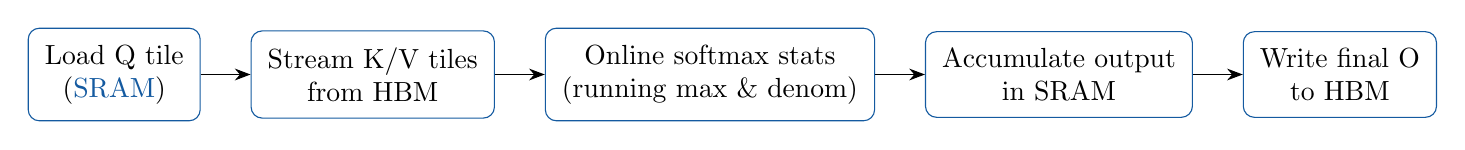
\begin{tikzpicture}[node distance=10pt]
    \node[draw=myblue, rounded corners, inner sep=6pt, align=center] (q) {Load Q tile\\(\blue{SRAM})};
    \node[draw=myblue, rounded corners, inner sep=6pt, align=center, right=18pt of q] (kv) {Stream K/V tiles\\from HBM};
    \node[draw=myblue, rounded corners, inner sep=6pt, align=center, right=18pt of kv] (soft) {Online softmax stats\\(running max \& denom)};
    \node[draw=myblue, rounded corners, inner sep=6pt, align=center, right=18pt of soft] (acc) {Accumulate output\\in SRAM};
    \node[draw=myblue, rounded corners, inner sep=6pt, align=center, right=18pt of acc] (write) {Write final O\\to HBM};
    
    \draw[-{Stealth[length=2mm]}] (q) -- (kv);
    \draw[-{Stealth[length=2mm]}] (kv) -- (soft);
    \draw[-{Stealth[length=2mm]}] (soft) -- (acc);
    \draw[-{Stealth[length=2mm]}] (acc) -- (write);
    \end{tikzpicture}
    \end{center}
    
    \begin{bluebox}
    \textbf{Why it works:} keep tiles in fast memory (\blue{SRAM}), do more compute per byte loaded, and avoid materializing the full attention matrix in HBM.
    \end{bluebox}
    
    % ---------------------------
    % Precision pitfalls (FP32 fallback)
    % ---------------------------
    \item \danger{FP32 fallback problem (why quantization/low-precision is tricky):}\\
    Some operations are sensitive and often require higher precision to stay numerically stable:
    \begin{itemize}
    \item softmax
    \item normalization layers
    \item attention score calculations
    \item reductions
    \end{itemize}
    
    % ---------------------------
    % Memory layout changes: INT4 example
    % ---------------------------
    \item \term{Memory layout changes (example: INT4):}\\
    \textbf{INT4} means two weights per byte. That forces you to:
    \begin{itemize}
    \item pack/unpack bits
    \item align memory correctly
    \item avoid warp divergence (branchy unpack logic can hurt)
    \end{itemize}
    
    \item \term{Warp divergence (clean definition):}\\
    Warp divergence occurs when threads within the same warp (typically 32 threads) follow different execution paths due to branches (\texttt{if/else}, loops). The GPU serializes the paths (masking off inactive threads), which reduces performance.
    
    % ---------------------------
    % Cluster slowdown checklist (cleaned)
    % ---------------------------
    \item \term{If code is slow on a cluster, check:}
    \begin{itemize}
    \item network filesystem latency
    \item improper CPU/GPU allocation (pinning, affinity, data loader threads)
    \item environment differences (drivers, CUDA version, library builds)
    \item container overhead / misconfiguration
    \item I/O contention (shared storage hot spots)
    \end{itemize}
    
    % ---------------------------
    % GPU memory hierarchy + scheduler note
    % ---------------------------
    \item \term{GPU memory hierarchy (fast recall):}\\
    GPUs have fast on-chip memory (registers, shared memory) and slower global memory (HBM/DRAM). Efficient kernels maximize locality and minimize global memory access.
    
    \item \term{Scheduler vs dispatcher:}\\
    Scheduler picks which warp runs; dispatcher issues the instruction to the pipelines/cores.
    
    % ---------------------------
    % Block size tradeoffs table (fixed + completed)
    % ---------------------------
    \item \term{Large blocks vs small blocks (tradeoffs):}
    \begin{center}
    \renewcommand{\arraystretch}{1.15}
    \begin{tabular}{|p{0.22\linewidth}|p{0.34\linewidth}|p{0.34\linewidth}|}
    \hline
    \textbf{Aspect} & \textbf{Large blocks} & \textbf{Small blocks} \\
    \hline
    Reuse / shared memory & Often higher (good tiling) & Often lower \\
    \hline
    Latency hiding & Can be worse if fewer warps fit & Often better (more runnable warps) \\
    \hline
    Global memory traffic & Often lower (reuse) & Often higher \\
    \hline
    Occupancy & May drop (regs/shared mem limit blocks) & May rise (more blocks fit) \\
    \hline
    \end{tabular}
    \end{center}
    
    % ---------------------------
    % GPU terms table (cleaned)
    % ---------------------------
    \item \term{GPU terms (in your words, clarified):}
    \begin{center}
    \renewcommand{\arraystretch}{1.15}
    \begin{tabular}{|p{0.20\linewidth}|p{0.72\linewidth}|}
    \hline
    \textbf{Term} & \textbf{Meaning (your wording, clarified)} \\
    \hline
    Block & A block of threads/tasks scheduled onto one SM (like a “work unit”). \\
    \hline
    Warp & Fixed group of 32 threads (SIMT unit) scheduled together. \\
    \hline
    Warp scheduler & Chooses which warp issues instructions each cycle. \\
    \hline
    Dispatcher & Sends the chosen warp’s instruction into the pipelines/cores. \\
    \hline
    GigaThread engine & Higher-level manager coordinating blocks across SMs (global scheduling). \\
    \hline
    \end{tabular}
    \end{center}
    
    % ---------------------------
    % Zoomed-out GPU picture (cleaned)
    % ---------------------------
    \item \term{Zooming out: whole GPU picture (Ampere/Hopper-class systems):}
    \begin{itemize}
    \item \term{PCIe:} host interface (bus moving data between host and device).
    \item \term{NVLink:} high-bandwidth interconnect between GPUs.
    \end{itemize}
    
    \textbf{Latency comparison (slow $\rightarrow$ fast):}\\
    Global memory $<$ L2 $<$ L1 / Shared $<$ Registers $<$ FMA $<$ Tensor Cores
    
    \begin{bluebox}
    \textbf{Practical takeaway:} hide memory latency and network communication (often the slow parts).
    \end{bluebox}
    
    \item \term{Arithmetic intensity (repeat, because it’s that important):}\\
    Arithmetic intensity $=$ FLOPs / bytes moved over HBM (device memory). Compute via profiling and compare to hardware:
    \begin{itemize}
    \item If workload ratio $<$ hardware ratio $\Rightarrow$ not compute-bound (likely memory or network-bound).
    \item If workload ratio $\approx$ hardware ratio $\Rightarrow$ likely compute-bound (need better kernels or more GPUs).
    \end{itemize}
    
    \item \term{MFU (Model FLOPs Utilization):} value in $[0,1]$ = actual FLOPs achieved / achievable FLOPs on hardware.
    
    % ---------------------------
    % Interconnect cheat table
    % ---------------------------
    \item \term{Interconnect cheat sheet:}
    \begin{center}
    \renewcommand{\arraystretch}{1.15}
    \begin{tabular}{|p{0.18\linewidth}|p{0.30\linewidth}|p{0.44\linewidth}|}
    \hline
    \textbf{Tech} & \textbf{Connects} & \textbf{Why it matters} \\
    \hline
    PCIe & CPU/host $\leftrightarrow$ GPU & host-device bandwidth/latency bottleneck \\
    \hline
    NVLink & GPU $\leftrightarrow$ GPU & high bandwidth for multi-GPU on-node \\
    \hline
    InfiniBand/RDMA & node $\leftrightarrow$ node & faster distributed training communication \\
    \hline
    GPUDirect RDMA & GPU $\leftrightarrow$ NIC & avoids host copies (lower latency, less CPU overhead) \\
    \hline
    \end{tabular}
    \end{center}
    
    % ---------------------------
    % CUDA mapping (fast recall)
    % ---------------------------
    \item \term{CUDA mapping (fast recall):}\\
    Grid $\rightarrow$ many blocks across the GPU \quad
    Block $\rightarrow$ runs on one SM \quad
    Warp $\rightarrow$ 32 threads scheduled together
    
    % ---------------------------
    % NCCL + collectives table (completed + formatted)
    % ---------------------------
    \item \term{NCCL (collective communication library):}\\
    Rank is a unique identifier for a GPU (e.g., one node broadcasts weights to all others).
    
    \begin{center}
    \renewcommand{\arraystretch}{1.15}
    \begin{tabular}{|p{0.18\linewidth}|p{0.46\linewidth}|p{0.28\linewidth}|}
    \hline
    \textbf{Collective} & \textbf{What it does (your wording, clarified)} & \textbf{Common use} \\
    \hline
    Broadcast & One rank sends data to all other ranks & weights/config \\
    \hline
    AllReduce & Reduce across all ranks and store result in every rank’s buffer & gradient sync (DP) \\
    \hline
    Reduce & Reduce across ranks; result stored in one rank & aggregation \\
    \hline
    AllGather & Gather shards so every rank ends with the full data & unshard (FSDP) \\
    \hline
    ReduceScatter & Reduce, then scatter shards so each rank keeps only a shard & FSDP grads \\
    \hline
    \end{tabular}
    \end{center}
    
    Used for gradient sync (data-parallel training): each GPU has a model replica, runs a separate mini-batch, does forward + backward, produces partial gradients, then synchronizes gradients and applies the weight update.
    
    AllGather (preserved + clarified): used when parameters/activations are sharded across devices; you may need to unshard so everything is available for a step.
    
    ReduceScatter (preserved + clarified): instead of every rank having a full copy, each rank keeps only a shard of the reduced result (common in FSDP). After the update, you often AllGather again.
    
    % ---------------------------
    % Networking + storage tables (as-is but cleaned)
    % ---------------------------
    \item \term{Networks in a data center (quick table):}
    \begin{center}
    \renewcommand{\arraystretch}{1.15}
    \begin{tabular}{|p{0.18\linewidth}|p{0.40\linewidth}|p{0.34\linewidth}|}
    \hline
    \textbf{Network} & \textbf{Purpose} & \textbf{Key requirements} \\
    \hline
    Compute & GPU$\leftrightarrow$GPU traffic (training/inference) & low latency, high throughput, scalable \\
    \hline
    In-band mgmt & SSH, scheduling, repos, config & reliable, secure isolation, moderate BW \\
    \hline
    OOB mgmt & manage server if OS down (BMC) & always on, strong access control \\
    \hline
    \end{tabular}
    \end{center}
    
    \item \term{Tiered storage (quick table):}
    \begin{center}
    \renewcommand{\arraystretch}{1.15}
    \begin{tabular}{|p{0.18\linewidth}|p{0.46\linewidth}|p{0.28\linewidth}|}
    \hline
    \textbf{Tier} & \textbf{Used for} & \textbf{Tradeoff} \\
    \hline
    Local NVMe & hot data + fast scratch I/O & fastest, limited capacity \\
    \hline
    Parallel FS & shared high-speed access & scalable, more complex \\
    \hline
    NFS & configs/scripts/small data & simple, not for heavy throughput \\
    \hline
    Object store & checkpoints/logs/big datasets & durable + cheap, higher latency \\
    \hline
    \end{tabular}
    \end{center}
    
    % ---------------------------
    % NVIDIA stack layers (cleaned list)
    % ---------------------------
    \item \term{Layers in NVIDIA infrastructure (clean list):}
    \begin{enumerate}[leftmargin=1.2em]
    \item Physical layer: GPU, data center, NICs, DPU
    \item Data movement \& I/O acceleration: NVLink, RDMA, storage, HPC fabrics (InfiniBand)
    \item OS / drivers / virtualization: GPU drivers
    \item Core libraries: CUDA, NCCL
    \item Monitoring \& management: NVIDIA-SMI, etc.
    \item Applications / vertical solutions: NVIDIA NIMs, enterprise stacks
    \end{enumerate}
    
    % ---------------------------
    % vGPU vs MIG + GPUDirect quick tables (preserved)
    % ---------------------------
    \item \term{GPUDirect summary (quick table):}
    \begin{center}
    \renewcommand{\arraystretch}{1.15}
    \begin{tabular}{|p{0.24\linewidth}|p{0.44\linewidth}|p{0.26\linewidth}|}
    \hline
    \textbf{Feature} & \textbf{Connects} & \textbf{Goal} \\
    \hline
    GPUDirect RDMA & GPU mem $\leftrightarrow$ NIC $\leftrightarrow$ network $\leftrightarrow$ NIC $\leftrightarrow$ GPU mem & low latency, avoid CPU copies \\
    \hline
    GPUDirect Storage & GPU mem $\leftrightarrow$ NVMe / storage fabric & feed GPUs faster (I/O) \\
    \hline
    \end{tabular}
    \end{center}
    
    \item \term{vGPU vs MIG (quick table):}
    \begin{center}
    \renewcommand{\arraystretch}{1.15}
    \begin{tabular}{|p{0.16\linewidth}|p{0.34\linewidth}|p{0.42\linewidth}|}
    \hline
    \textbf{Tech} & \textbf{Isolation} & \textbf{Typical usage} \\
    \hline
    vGPU & software-enforced (hypervisor) & VM environments, cloud multi-tenant VMs \\
    \hline
    MIG & hardware-enforced & containers, HPC/AI clusters, strong partitioning \\
    \hline
    \end{tabular}
    \end{center}
    
    % ---------------------------
    % BCM preserved + cleaned (you had an abrupt ending)
    % ---------------------------
    \item \term{BCM (Base Command Manager):}\\
    Manage, monitor, and orchestrate GPU resources and workloads across an entire AI data center (cluster utilization, infra health, job status, quotas, workload performance).
    
    \begin{itemize}
    \item \blue{Management/config:} firmware configs, power policies, provisioning, scheduling, allocation, deployments.
    \item \blue{Monitoring:} CPU, GPUs, networking, storage, workloads (AI/HPC).
    \item Interfaces: CLI, web UI, REST API.
    \end{itemize}
    
\end{itemize}

%%%%%%%%%%%%%%%%%%%%%%%%%%%%%%%%%%%%%%%%%%%%%%%%%%%%%%%%%%%%
\section{Code Snippets I Should Know}
%%%%%%%%%%%%%%%%%%%%%%%%%%%%%%%%%%%%%%%%%%%%%%%%%%%%%%%%%%%%

\begin{bluebox}
\textbf{Goal:} be able to name the \blue{tool}, \blue{what it tells you}, and \red{when you’d use it} in an interview.
\end{bluebox}

%%%%%%%%%%%%%%%%%%%%%%%%%%%%%%%%%%%%%%%%%%%%%%%%%%%%%%%%%%%%
% 1) PROFILING + DEBUGGING TOOLS (cleaned + organized)
%%%%%%%%%%%%%%%%%%%%%%%%%%%%%%%%%%%%%%%%%%%%%%%%%%%%%%%%%%%%
\subsection{Profiling / Debugging Cheat Sheet}

\begin{center}
\renewcommand{\arraystretch}{1.2}
\begin{tabular}{|p{0.26\linewidth}|p{0.64\linewidth}|}
\hline
\textbf{Tool / Snippet} & \textbf{Meaning (clean + interview-ready)} \\
\hline
\blue{\textbf{Nsight Systems (nsys)}} & End-to-end timeline: CPU$\leftrightarrow$GPU overlap, kernel launches, synchronization, memcpy, data loader stalls. \\
\hline
\blue{\textbf{Nsight Compute (ncu)}} & Deep kernel analysis: occupancy, memory throughput, instruction mix, warp stalls, cache behavior. \\
\hline
\blue{\textbf{cuda-gdb}} & Debug CUDA kernels (breakpoints, stepping, inspecting variables). \\
\hline
\blue{\textbf{cuda-memcheck}} & Memory correctness: out-of-bounds, invalid accesses, (some) race-like issues. \\
\hline
\blue{\textbf{CUDA runtime + driver APIs}} &
Managing devices, memory, and program execution on the GPU. \\
\hline
\blue{\textbf{cudaMalloc(\dots)}} & Allocates memory on the \textbf{GPU}. (\texttt{malloc} allocates on \textbf{CPU}.) \\
\hline
\blue{\textbf{cudaMemcpy(\dots)}} & Copies data \textbf{CPU$\leftrightarrow$GPU} (host-device transfers). \\
\hline
\end{tabular}
\end{center}

\begin{redbox}
\textbf{Fast rule:} \blue{nsys} tells you \emph{where time goes overall}. \blue{ncu} tells you \emph{why a specific kernel is slow}.
\end{redbox}

%%%%%%%%%%%%%%%%%%%%%%%%%%%%%%%%%%%%%%%%%%%%%%%%%%%%%%%%%%%%
% 2) NVIDIA-SMI COMMANDS (cleaned + completed + permission note)
%%%%%%%%%%%%%%%%%%%%%%%%%%%%%%%%%%%%%%%%%%%%%%%%%%%%%%%%%%%%
\subsection{NVIDIA-SMI (Node Monitoring)}

\begin{center}
\renewcommand{\arraystretch}{1.2}
\begin{tabular}{|p{0.34\linewidth}|p{0.56\linewidth}|}
\hline
\textbf{What you want} & \textbf{Command} \\
\hline
Show summary (default view) & \texttt{nvidia-smi} \\
\hline
Refresh every 1 second & \texttt{nvidia-smi -l 1} \\
\hline
Show specific fields (custom query) &
\texttt{nvidia-smi --query-gpu=name,uuid,utilization.gpu,utilization.mem --format=csv} \\
\hline
Save full report to a file &
\texttt{nvidia-smi -q > smi\_report.txt} \\
\hline
Check clocks in use (graphics/SM/memory) &
\texttt{nvidia-smi -q -d CLOCK} \\
\hline
Check all supported clocks &
\texttt{nvidia-smi -q -d SUPPORTED\_CLOCKS} \\
\hline
Set power limit (requires permission) &
\texttt{sudo nvidia-smi -pl 200} \\
\hline
Set application clocks (if supported + permitted) &
\texttt{sudo nvidia-smi -ac <memClockMHz>,<smClockMHz>} \\
\hline
Why it might fail (permission note) &
If you see \red{\textbf{Insufficient Permissions}}, you need admin/sudo access or the cluster must allow user-level power/clock controls. \\
\hline
\end{tabular}
\end{center}

%%%%%%%%%%%%%%%%%%%%%%%%%%%%%%%%%%%%%%%%%%%%%%%%%%%%%%%%%%%%
% 3) NCU QUICK COMMANDS (completed INSERT with real commands)
%%%%%%%%%%%%%%%%%%%%%%%%%%%%%%%%%%%%%%%%%%%%%%%%%%%%%%%%%%%%
\subsection{Nsight Compute (NCU) Quick Commands}

\begin{bluebox}
\textbf{Use NCU to answer:} am I \blue{compute-bound} or \blue{memory-bound}, and what limits occupancy/stalls?
\end{bluebox}

\begin{center}
\renewcommand{\arraystretch}{1.2}
\begin{tabular}{|p{0.38\linewidth}|p{0.52\linewidth}|}
\hline
\textbf{What you want} & \textbf{Command} \\
\hline
Profile app (basic) & \texttt{ncu ./vecAdd} \\
\hline
Fuller kernel metrics (heavier) & \texttt{ncu --set full ./vecAdd} \\
\hline
Profile only one kernel by name & \texttt{ncu -k vecAdd ./vecAdd} \\
\hline
Save report file & \texttt{ncu -o report\_vecAdd ./vecAdd} \\
\hline
Reduce overhead (often faster) & \texttt{ncu --replay-mode application ./vecAdd} \\
\hline
\end{tabular}
\end{center}

%%%%%%%%%%%%%%%%%%%%%%%%%%%%%%%%%%%%%%%%%%%%%%%%%%%%%%%%%%%%
% 4) CUDA INDEXING QUICK RECALL (cleaned)
%%%%%%%%%%%%%%%%%%%%%%%%%%%%%%%%%%%%%%%%%%%%%%%%%%%%%%%%%%%%
\subsection{CUDA Indexing (Fast Recall)}

\begin{center}
\renewcommand{\arraystretch}{1.2}
\begin{tabular}{|p{0.30\linewidth}|p{0.60\linewidth}|}
\hline
\textbf{Name} & \textbf{Meaning} \\
\hline
\texttt{gridDim.x}, \texttt{gridDim.y} & How many blocks wide/tall in the launched grid. \\
\hline
\texttt{blockDim.x}, \texttt{blockDim.y} & Threads per block in x/y. \\
\hline
\texttt{threadIdx.x}, \texttt{threadIdx.y} & Thread’s local coordinates inside its block. \\
\hline
\texttt{blockIdx.x}, \texttt{blockIdx.y} & Block’s coordinates inside the grid. \\
\hline
\end{tabular}
\end{center}

\begin{bluebox}
\textbf{2D output indexing (matmul / conv-style):}\\
\[
i = \texttt{blockIdx.y}\cdot\texttt{blockDim.y} + \texttt{threadIdx.y},
\qquad
j = \texttt{blockIdx.x}\cdot\texttt{blockDim.x} + \texttt{threadIdx.x}
\]
\end{bluebox}

%%%%%%%%%%%%%%%%%%%%%%%%%%%%%%%%%%%%%%%%%%%%%%%%%%%%%%%%%%%%
% 5) SLURM srun line breakdown (completed INSERT)
%%%%%%%%%%%%%%%%%%%%%%%%%%%%%%%%%%%%%%%%%%%%%%%%%%%%%%%%%%%%
\subsection{Cluster Launch (Slurm) — \texttt{srun} Line Breakdown}

\begin{bluebox}
\textbf{Command (preserved):}\\
\texttt{srun --partition=gpu --gres=gpu:1 --mem=16G --time=01:00:00 --pty bash}
\end{bluebox}

\begin{center}
\renewcommand{\arraystretch}{1.2}
\begin{tabular}{|p{0.30\linewidth}|p{0.60\linewidth}|}
\hline
\textbf{Flag} & \textbf{What it does} \\
\hline
\texttt{--partition=gpu} & Run on the GPU partition/queue. \\
\hline
\texttt{--gres=gpu:1} & Request 1 GPU resource. \\
\hline
\texttt{--mem=16G} & Request 16 GB of system RAM. \\
\hline
\texttt{--time=01:00:00} & Time limit of 1 hour. \\
\hline
\texttt{--pty bash} & Start an interactive pseudo-terminal (a shell) on the allocated node. \\
\hline
\end{tabular}
\end{center}

\begin{redbox}
\textbf{Interview phrasing:} “\texttt{srun --pty} is how I grab an interactive GPU node to debug quickly before running a long \texttt{sbatch} job.”
\end{redbox}

%%%%%%%%%%%%%%%%%%%%%%%%%%%%%%%%%%%%%%%%%%%%%%%%%%%%%%%%%%%%
% 6) NAIVE MATMUL: CPU + CUDA (completed INSERT)
%%%%%%%%%%%%%%%%%%%%%%%%%%%%%%%%%%%%%%%%%%%%%%%%%%%%%%%%%%%%
\subsection{Naive Matrix Multiply (CPU + CUDA) — Interview Baseline}

\begin{bluebox}
\textbf{Purpose:} show you understand indexing, memory layout, and where the bottleneck comes from.  
This is \red{naive} (no tiling/shared memory). Optimizations come after.
\end{bluebox}

\subsubsection*{\blue{CPU Naive Matmul (row-major)}}
\begin{verbatim}
void matmul_cpu(const float* A, const float* B, float* C,
                int M, int K, int N) {
  // A: MxK, B: KxN, C: MxN (row-major)
  for (int i = 0; i < M; i++) {
    for (int j = 0; j < N; j++) {
      float sum = 0.0f;
      for (int k = 0; k < K; k++) {
        sum += A[i*K + k] * B[k*N + j];
      }
      C[i*N + j] = sum;
    }
  }
}
\end{verbatim}

\subsubsection*{\blue{CUDA Naive Matmul Kernel}}
\begin{verbatim}
__global__ void matmul_cuda(const float* A, const float* B, float* C,
                            int M, int K, int N) {
  int i = blockIdx.y * blockDim.y + threadIdx.y; // row
  int j = blockIdx.x * blockDim.x + threadIdx.x; // col

  if (i < M && j < N) {
    float sum = 0.0f;
    for (int k = 0; k < K; k++) {
      sum += A[i*K + k] * B[k*N + j];
    }
    C[i*N + j] = sum;
  }
}
\end{verbatim}

\subsubsection*{\blue{Launch Configuration (simple)}}
\begin{verbatim}
// Example: 16x16 threads per block
dim3 block(16, 16);
dim3 grid((N + block.x - 1) / block.x,
          (M + block.y - 1) / block.y);

matmul_cuda<<<grid, block>>>(A, B, C, M, K, N);
\end{verbatim}

\begin{redbox}
\textbf{What makes this naive kernel slow:}
\begin{itemize}
\item Each thread re-loads A/B from global memory many times (low data reuse).
\item No shared-memory tiling, so memory traffic is high.
\item Typically becomes \blue{memory-bound} at scale (unless extremely small sizes).
\end{itemize}
\end{redbox}

%%%%%%%%%%%%%%%%%%%%%%%%%%%%%%%%%%%%%%%%%%%%%%%%%%%%%%%%%%%%
% Interview Memory Table (match style of sections above)
%%%%%%%%%%%%%%%%%%%%%%%%%%%%%%%%%%%%%%%%%%%%%%%%%%%%%%%%%%%%

\subsection{Interview Memory Table: NN Concepts + How They Connect}

\begin{bluebox}
\textbf{Goal:} quick recall for interviews — \blue{definition} + \red{how it connects} in training/inference.
\end{bluebox}

\renewcommand{\arraystretch}{1.2}
\setlength{\tabcolsep}{6pt}
\begin{longtable}{|p{0.16\linewidth}|p{0.24\linewidth}|p{0.50\linewidth}|}
\hline
\blue{\textbf{Concept}} & \blue{\textbf{What it is (1-liner)}} & \red{\textbf{How it relates to everything else}} \\
\hline

\textbf{Weights} ($W$) &
Learned parameters that scale/combine input features. &
Used in the \textbf{forward pass} to compute $z = Wx + b$; updated in \textbf{backprop} via gradients $\nabla_W \mathcal{L}$; influenced by \textbf{initialization} and \textbf{regularization} (e.g., weight decay); \textbf{batch norm} can change effective scaling. \\
\hline

\textbf{Biases} ($b$) &
Learned offsets that shift activations. &
Also used in forward pass $z = Wx + b$; gradients $\nabla_b \mathcal{L}$ computed in backprop; often less regularized than $W$; interacts with \textbf{batch norm} (BN can reduce the need for explicit biases). \\
\hline

\textbf{Activation} ($\sigma$) &
Nonlinearity applied to $z$ (e.g., ReLU, sigmoid). &
Makes networks expressive; in \textbf{backprop} you multiply by $\sigma'(z)$ (chain rule); affects gradient flow (vanishing/exploding) and drives good \textbf{initialization} choices. \\
\hline

\textbf{Forward pass} &
Compute predictions from inputs. &
Pipeline: input $\rightarrow$ (optional \textbf{BN}) $\rightarrow$ linear ($W,b$) $\rightarrow$ \textbf{activation} $\rightarrow$ (optional \textbf{pooling}) $\rightarrow \hat{y}$; stores activations needed for the \textbf{backward pass}. \\
\hline

\textbf{Loss} ($\mathcal{L}$) &
Measures prediction error (e.g., cross-entropy, MSE). &
Backprop computes gradients of $\mathcal{L}$ w.r.t.\ parameters; may include \textbf{regularization}: $\mathcal{L}_{\text{total}} = \mathcal{L}_{\text{data}} + \lambda R(W)$; drives \textbf{gradient descent} updates. \\
\hline

\textbf{Backprop} &
Compute gradients using the chain rule. &
Uses saved forward activations; outputs $\nabla_W\mathcal{L}$, $\nabla_b\mathcal{L}$, etc.; gradients are consumed by the \textbf{optimizer}; stability depends on \textbf{activation}, \textbf{initialization}, and \textbf{BN}. \\
\hline

\textbf{Gradient descent} &
Update rule: move parameters opposite the gradient. &
Core update: $W \leftarrow W - \eta \nabla_W \mathcal{L}$; $\eta$ is the \textbf{learning rate}; most \textbf{optimizers} are improved variants (momentum/adaptive steps). \\
\hline

\textbf{Learning rate} ($\eta$) &
Step size for parameter updates. &
Too big $\Rightarrow$ divergence; too small $\Rightarrow$ slow training; interacts with \textbf{optimizer} (Adam often tolerates larger $\eta$ than SGD), \textbf{BN} (stabilizes), and \textbf{regularization} (effective update size changes). \\
\hline

\textbf{Optimizer} &
Algorithm that uses gradients to update parameters (SGD, Adam, etc.). &
Consumes gradients from backprop; may add momentum/adaptive scaling/weight decay; strongly interacts with \textbf{learning rate} and \textbf{regularization}; determines training dynamics and convergence speed. \\
\hline

\textbf{Regularization} &
Techniques to reduce overfitting (L2, dropout, etc.). &
Often added to loss (e.g., L2: $\lambda \lVert W\rVert^2$), changing gradients; constrains weight growth (helps stability); interacts with optimizer (e.g., AdamW decouples weight decay). \\
\hline

\textbf{Initialization} &
How you set starting values of $W,b$. &
Sets early signal/gradient scales; poor init $\Rightarrow$ vanishing/exploding gradients; chosen based on \textbf{activation} (He for ReLU, Xavier for tanh/sigmoid-ish). \\
\hline

\textbf{Batch Norm (BN)} &
Normalizes activations using batch statistics. &
Inserted in forward pass; changes gradient flow in backprop; stabilizes training, allows higher \textbf{learning rate}, reduces sensitivity to \textbf{initialization}; adds learnable scale/shift ($\gamma,\beta$). \\
\hline

\textbf{Pooling} &
Downsamples spatial features (CNNs). &
Part of forward pass after conv/activation; reduces compute and adds invariance; in backprop routes gradients (max $\rightarrow$ argmax only, avg $\rightarrow$ distributed). \\
\hline

\end{longtable}

\begin{redbox}
\textbf{Interview pattern:} \blue{Forward pass creates activations} $\rightarrow$ \blue{loss measures error} $\rightarrow$ \blue{backprop computes gradients} $\rightarrow$ \blue{optimizer updates $W,b$} (controlled by \blue{$\eta$} and \blue{regularization}).
\end{redbox}

%%%%%%%%%%%%%%%%%%%%%%%%%%%%%%%%%%%%%%%%%%%%%%%%%%%%%%%%%%%%%%%%%%%%%%%%%%%%%%%%%%%%%%%%%%%%%%%%%%%%%%%%%%%%%%%%%%%%%%%%
\section{Serving an LLM (Table Summary)}
%%%%%%%%%%%%%%%%%%%%%%%%%%%%%%%%%%%%%%%%%%%%%%%%%%%%%%%%%%%%%%%%%%%%%%%%%%%%%%%%%%%%%%%%%%%%%%%%%%%%%%%%%%%%%%%%%%%%%%%%

\begin{bluebox}
\textbf{Big idea:} Serving an LLM means turning a trained model into a
\blue{fast, reliable API} that real applications can call.
\end{bluebox}

\vspace{0.5em}

\renewcommand{\arraystretch}{1.25}
\setlength{\tabcolsep}{6pt}

\begin{tabular}{|p{3.3cm}|p{5.6cm}|p{6.2cm}|}
\hline
\textbf{Stage} & \textbf{What Happens} & \textbf{Key Points / Interview Memory} \\
\hline

Freeze Model &
Save weights, tokenizer, configs; lock versions. &
Start with \blue{FP16/BF16}; use \red{quantization} later if memory/latency matters. Ensures reproducibility and stable deployment. \\
\hline

Inference Engine &
Software that loads model onto GPUs and serves requests. &
Example: \textbf{vLLM} — efficient batching, KV-cache optimization, high throughput. Provides API endpoint for apps. \\
\hline

Chain / App Layer &
Business logic between app and model. &
Build prompts, call tools (DB/search/code), format outputs, retries, moderation. Often FastAPI/Node. \\
\hline

RAG (Optional) &
External knowledge retrieval before generation. &
Chunk docs $\rightarrow$ embeddings $\rightarrow$ vector DB $\rightarrow$ retrieve relevant text $\rightarrow$ add to prompt.  
\textbf{Memory idea:} \red{Search first, then generate.} \\
\hline

Production Architecture &
Typical serving pipeline. &
App $\rightarrow$ API Gateway $\rightarrow$ Chain Service $\rightarrow$ LLM Server $\rightarrow$ GPU. Separates concerns for scalability. \\
\hline

Production Concerns &
Operational considerations. &
\blue{Latency:} TTFT, tokens/sec.  
\blue{GPU usage:} memory/utilization.  
\blue{Scaling:} batching, multi-GPU.  
\red{Safety:} moderation, injection defense.  
\blue{Reliability:} monitoring, retries. \\
\hline

Deployment Options &
Infrastructure scale choices. &
Single GPU (simple dev), multi-GPU node (higher throughput), distributed multi-node serving (large scale). \\
\hline

\end{tabular}

\vspace{0.6em}

\begin{bluebox}
\textbf{Interview one-liner:}

\textit{“Serving an LLM means freezing the model,
running it behind an optimized inference server,
adding business logic or RAG in front,
and monitoring latency, GPU usage, and reliability in production.”}
\end{bluebox}
%%%%%%%%%%%%%%%%%%%%%%%%%%%%%%%%%%%%%%%%%%%%%%%%%%%%%%%%%%%%
% FILLED PROJECT NOTES — NVIDIA / HPC / DL INFRA FOCUS
%%%%%%%%%%%%%%%%%%%%%%%%%%%%%%%%%%%%%%%%%%%%%%%%%%%%%%%%%%%%

%%%%%%%%%%%%%%%%%%%%%%%%%%%%%%%%%%%%%%%%%%%%%%%%%%%%%%%%%%%%
\ProjectHeader{Research: Evaluation of Optimization Techniques for Large Language Model Inference}{LLM inference frameworks, profiling, quantization, batching, GPU performance}
%%%%%%%%%%%%%%%%%%%%%%%%%%%%%%%%%%%%%%%%%%%%%%%%%%%%%%%%%%%%

\subsection{Short Pitch (GPU / HPC Focus)}
Studied performance bottlenecks in LLM inference pipelines across different runtimes,
focusing on GPU utilization, memory bandwidth, batching strategies, and quantization.
Goal was understanding how to maximize throughput on modern GPU clusters.

\subsection{Why I Did It + What I Learned}
\begin{itemize}
\item Wanted deeper intuition for inference bottlenecks beyond training.
\item Learned how KV-cache behavior, batching, and memory bandwidth dominate LLM serving.
\item Built strong understanding of arithmetic intensity and GPU utilization tradeoffs.
\end{itemize}

\subsection{Challenges}
\begin{itemize}
\item Separating compute-bound vs memory-bound inference stages.
\item Interpreting profiler output across different frameworks.
\item Understanding scaling effects in multi-GPU serving setups.
\end{itemize}

\subsection{Key Interview Takeaways}
\begin{itemize}
\item GPU inference is often memory-bound, not compute-bound.
\item Batching + KV cache efficiency heavily impact throughput.
\item Expect questions on quantization, kernel efficiency, and GPU memory layout.
\end{itemize}

%%%%%%%%%%%%%%%%%%%%%%%%%%%%%%%%%%%%%%%%%%%%%%%%%%%%%%%%%%%%
\ProjectHeader{Convolutional Layer Optimization with Triton}{Triton, CUDA, PyTorch, GPU kernels}
%%%%%%%%%%%%%%%%%%%%%%%%%%%%%%%%%%%%%%%%%%%%%%%%%%%%%%%%%%%%

\subsection{Short Pitch}
Implemented custom Triton kernels to optimize 2D convolution layers,
reducing kernel overhead and improving GPU utilization compared to standard PyTorch ops.

\subsection{Why I Did It + What I Learned}
\begin{itemize}
\item Wanted hands-on experience writing GPU kernels for deep learning workloads.
\item Learned tiling strategies, memory coalescing, and warp-level execution effects.
\item Gained intuition for tensor core usage and instruction scheduling.
\end{itemize}

\subsection{Challenges}
\begin{itemize}
\item Achieving good occupancy without exceeding register/shared memory limits.
\item Debugging kernel correctness and performance simultaneously.
\item Balancing compute intensity with memory throughput.
\end{itemize}

\subsection{Key Interview Takeaways}
\begin{itemize}
\item Kernel optimization = memory locality + warp efficiency.
\item Profiling is essential (Nsight Compute).
\item Expect questions on tiling, occupancy, and tensor core usage.
\end{itemize}

%%%%%%%%%%%%%%%%%%%%%%%%%%%%%%%%%%%%%%%%%%%%%%%%%%%%%%%%%%%%
\ProjectHeader{LABUBU AI Shopper}{GPT-4, vector search, FastAPI, React, Faiss}
%%%%%%%%%%%%%%%%%%%%%%%%%%%%%%%%%%%%%%%%%%%%%%%%%%%%%%%%%%%%

\subsection{Short Pitch}
Built a real-time AI shopping assistant using vector search + LLM prompting,
handling ~1000 SKUs with sub-second response time.

\subsection{Why I Did It + What I Learned}
\begin{itemize}
\item Wanted production-style LLM system experience.
\item Learned prompt engineering, retrieval augmentation, and latency optimization.
\item Understood tradeoffs between embedding search cost and response speed.
\end{itemize}

\subsection{Challenges}
\begin{itemize}
\item Managing latency across retrieval + LLM inference pipeline.
\item Scaling vector search while maintaining response quality.
\item Designing reliable API integration.
\end{itemize}

\subsection{Key Interview Takeaways}
\begin{itemize}
\item Retrieval latency often dominates inference latency.
\item RAG pipelines require careful caching and batching.
\item Expect questions on LLM serving architecture.
\end{itemize}

%%%%%%%%%%%%%%%%%%%%%%%%%%%%%%%%%%%%%%%%%%%%%%%%%%%%%%%%%%%%
\ProjectHeader{GPU-Accelerated Image Processing Pipeline}{CUDA, PyTorch, V100 GPUs}
%%%%%%%%%%%%%%%%%%%%%%%%%%%%%%%%%%%%%%%%%%%%%%%%%%%%%%%%%%%%

\subsection{Short Pitch}
Built GPU-accelerated image filters (blur/sharpen) achieving ~8× speedup
over CPU baselines through CUDA parallelization.

\subsection{Why I Did It + What I Learned}
\begin{itemize}
\item Wanted strong GPU fundamentals before deeper ML systems work.
\item Learned kernel launch configuration, memory hierarchy, and profiling.
\item Developed intuition for when GPU acceleration is worthwhile.
\end{itemize}

\subsection{Challenges}
\begin{itemize}
\item Optimizing memory access patterns.
\item Avoiding unnecessary host-device transfers.
\item Achieving stable benchmarking.
\end{itemize}

\subsection{Key Interview Takeaways}
\begin{itemize}
\item Memory movement often dominates GPU pipelines.
\item Data locality strongly affects performance.
\item Expect questions on CUDA memory hierarchy.
\end{itemize}

%%%%%%%%%%%%%%%%%%%%%%%%%%%%%%%%%%%%%%%%%%%%%%%%%%%%%%%%%%%%
\ProjectHeader{High-Performance Matrix Inversion via GPU Kernels}{Triton, OpenCL, C++}
%%%%%%%%%%%%%%%%%%%%%%%%%%%%%%%%%%%%%%%%%%%%%%%%%%%%%%%%%%%%

\subsection{Short Pitch}
Implemented custom GPU kernels for large matrix inversion (~5000×5000),
achieving ~50\% runtime reduction versus CPU implementations.

\subsection{Why I Did It + What I Learned}
\begin{itemize}
\item Interest in HPC linear algebra performance optimization.
\item Learned parallel decomposition, kernel scheduling, and memory tiling.
\item Improved understanding of GPU numerical stability issues.
\end{itemize}

\subsection{Challenges}
\begin{itemize}
\item Managing numerical precision on GPU.
\item Ensuring stable performance scaling.
\item Avoiding excessive memory transfers.
\end{itemize}

\subsection{Key Interview Takeaways}
\begin{itemize}
\item Linear algebra dominates many ML workloads.
\item GPU kernels require careful tiling.
\item Expect HPC-style performance questions.
\end{itemize}

%%%%%%%%%%%%%%%%%%%%%%%%%%%%%%%%%%%%%%%%%%%%%%%%%%%%%%%%%%%%
\ProjectHeader{Parking Ticket Prevention Streaming Platform}{Spark, Kafka, Lambda}
%%%%%%%%%%%%%%%%%%%%%%%%%%%%%%%%%%%%%%%%%%%%%%%%%%%%%%%%%%%%

\subsection{Short Pitch}
Built a real-time streaming system tracking enforcement vehicles
and delivering proactive alerts using distributed event pipelines.

\subsection{Why I Did It + What I Learned}
\begin{itemize}
\item Wanted distributed systems experience.
\item Learned event streaming, fault tolerance, and scaling pipelines.
\item Improved understanding of latency vs throughput tradeoffs.
\end{itemize}

\subsection{Challenges}
\begin{itemize}
\item Managing streaming latency.
\item Coordinating multiple distributed services.
\item Ensuring reliability under load.
\end{itemize}

\subsection{Key Interview Takeaways}
\begin{itemize}
\item Distributed systems bottlenecks often shift to networking.
\item Monitoring is critical.
\item Expect system design questions.
\end{itemize}

%%%%%%%%%%%%%%%%%%%%%%%%%%%%%%%%%%%%%%%%%%%%%%%%%%%%%%%%%%%%
\ProjectHeader{HPC Workflows: Multi-GPU Training + Benchmarking}{Slurm, Kubernetes, profiling}
%%%%%%%%%%%%%%%%%%%%%%%%%%%%%%%%%%%%%%%%%%%%%%%%%%%%%%%%%%%%

\subsection{Short Pitch}
Designed HPC workflows supporting multi-GPU training,
cluster utilization optimization, and performance benchmarking.

\subsection{Why I Did It + What I Learned}
\begin{itemize}
\item Direct exposure to GPU cluster infrastructure.
\item Learned job scheduling, resource allocation, and profiling.
\item Developed intuition for distributed ML bottlenecks.
\end{itemize}

\subsection{Challenges}
\begin{itemize}
\item Load balancing across GPUs.
\item Debugging distributed training issues.
\item Maintaining reproducibility across environments.
\end{itemize}

\subsection{Key Interview Takeaways}
\begin{itemize}
\item Cluster utilization is often the biggest efficiency lever.
\item Communication overhead limits scaling.
\item Expect Slurm/Kubernetes/GPU scheduling questions.
\end{itemize}

%%%%%%%%%%%%%%%%%%%%%%%%%%%%%%%%%%%%%%%%%%%%%%%%%%%%%%%%%%%%
\ProjectHeader{Malware Detection Research}{PyTorch, ETL pipelines, synthetic data generation}
%%%%%%%%%%%%%%%%%%%%%%%%%%%%%%%%%%%%%%%%%%%%%%%%%%%%%%%%%%%%

\subsection{Short Pitch}
Developed ML-based malware detection workflows with synthetic data
generation and large-scale preprocessing pipelines.

\subsection{Why I Did It + What I Learned}
\begin{itemize}
\item Early ML research exposure.
\item Learned dataset engineering, imbalance handling, and ML pipelines.
\item Strengthened debugging and experimental design skills.
\end{itemize}

\subsection{Challenges}
\begin{itemize}
\item Class imbalance.
\item Data preprocessing at scale.
\item Model generalization.
\end{itemize}

\subsection{Key Interview Takeaways}
\begin{itemize}
\item Data quality often matters more than model complexity.
\item Scaling preprocessing is non-trivial.
\item Expect ML pipeline design questions.
\end{itemize}

%%%%%%%%%%%%%%%%%%%%%%%%%%%%%%%%%%%%%%%%%%%%%%%%%%%%%%%%%%%%
% FILLED PROJECT NOTES — NVIDIA / HPC / DL INFRA FOCUS
%%%%%%%%%%%%%%%%%%%%%%%%%%%%%%%%%%%%%%%%%%%%%%%%%%%%%%%%%%%%

%%%%%%%%%%%%%%%%%%%%%%%%%%%%%%%%%%%%%%%%%%%%%%%%%%%%%%%%%%%%
%%%%%%%%%%%%%%%%%%%%%%%%%%%%%%%%%%%%%%%%%%%%%%%%%%%%%%%%%%%%
\ProjectHeader{Research: Evaluation of Optimization Techniques for Large Language Model Inference}{LLMCompass, hardware benchmarking, inference optimization}
%%%%%%%%%%%%%%%%%%%%%%%%%%%%%%%%%%%%%%%%%%%%%%%%%%%%%%%%%%%%

\subsection{Short Pitch}
This research focused on understanding how large language model inference performance varies across different GPU hardware using the LLMCompass computational graph framework. LLMCompass models the inference pipeline as a computational graph and estimates how different GPUs handle memory bandwidth, compute throughput, and communication overhead. I analyzed how architectural factors like tensor core throughput, memory hierarchy, and interconnect bandwidth influence real inference performance rather than just theoretical FLOPs.

\subsection{Why I Did It + What I Learned}
I was interested in how hardware architecture impacts deep learning inference performance, especially for large language models deployed on GPU clusters. By studying the LLMCompass codebase, I learned how computational graphs can simulate inference workloads across different hardware configurations. I focused on understanding how memory movement, kernel scheduling, and arithmetic intensity determine bottlenecks. This helped me build intuition about why inference often becomes memory-bound and how batching, quantization, and kernel fusion improve throughput.

\subsection{Challenges}
The main challenge was interpreting the modeling assumptions in the LLMCompass framework and connecting them to real GPU behavior. I spent time tracing how the computational graph represented operations like attention, matrix multiplication, and KV-cache updates, then compared predicted performance with expected hardware characteristics. Understanding how communication overhead scales across GPUs was also non-trivial.

\subsection{Key Interview Takeaways}
This work reinforced that theoretical FLOPs rarely translate directly to real inference speed; memory bandwidth and data movement dominate. It also strengthened my understanding of hardware-aware model optimization and how profiling tools and simulation frameworks can guide deployment decisions.


%%%%%%%%%%%%%%%%%%%%%%%%%%%%%%%%%%%%%%%%%%%%%%%%%%%%%%%%%%%%
\ProjectHeader{Convolutional Layer Optimization with Triton}{Triton, CUDA concepts, PyTorch kernels}
%%%%%%%%%%%%%%%%%%%%%%%%%%%%%%%%%%%%%%%%%%%%%%%%%%%%%%%%%%%%

\subsection{Short Pitch}
In this project, I implemented optimized convolution kernels using Triton to accelerate 2D convolution layers commonly used in deep learning workloads. The goal was to improve GPU utilization by controlling memory tiling, thread mapping, and kernel execution rather than relying solely on high-level PyTorch primitives in CuDNN.

\subsection{Why I Did It + What I Learned}
I wanted hands-on experience writing GPU kernels to better understand performance bottlenecks in deep learning workloads. Writing Triton kernels helped me understand how threads map to data tiles, how shared memory and registers reduce global memory access, and how warp-level execution impacts efficiency. I also gained experience profiling GPU kernels and interpreting occupancy and throughput metrics.

\subsection{Technical Implementation (Code Logic)}
The kernel divides convolution output tensors into tiles so each GPU thread block computes a small portion of the output. Threads collaboratively load input feature maps and filters into faster on-chip memory, perform multiply–accumulate operations, and write results back to global memory. This tiling strategy increases arithmetic intensity by reusing data already loaded into shared memory. The kernel also carefully aligns memory accesses so adjacent threads access adjacent memory locations, improving coalescing and reducing bandwidth waste.

\subsection{Challenges}
Balancing occupancy with register and shared memory usage was the main challenge. Larger tiles improve data reuse but can reduce the number of concurrent warps. Debugging correctness while optimizing performance also required iterative profiling.

\subsection{Key Interview Takeaways}
GPU performance optimization often comes down to memory locality, tiling strategy, and efficient warp scheduling. Understanding how kernels map computation onto hardware is essential for deep learning inference optimization.


%%%%%%%%%%%%%%%%%%%%%%%%%%%%%%%%%%%%%%%%%%%%%%%%%%%%%%%%%%%%
\ProjectHeader{GPU-Accelerated Image Processing Pipeline}{CUDA, PyTorch, C++, NVIDIA GPUs}
%%%%%%%%%%%%%%%%%%%%%%%%%%%%%%%%%%%%%%%%%%%%%%%%%%%%%%%%%%%%

\subsection{Short Pitch}
This project implemented GPU-accelerated image filters such as blur and sharpen operations using CUDA, achieving significant speedups compared to CPU implementations by parallelizing pixel-level operations across thousands of GPU threads.

\subsection{Why I Did It + What I Learned}
I wanted foundational GPU programming experience before working on larger ML infrastructure problems. This project helped me understand CUDA kernel launches, thread indexing, memory hierarchies, and profiling workflows.

\subsection{Technical Implementation (Code Logic)}
Each CUDA thread processes a small region of the image, computing convolution-style filter operations independently. The kernel calculates pixel indices based on block and thread IDs, loads neighboring pixels needed for filtering, performs weighted averaging or sharpening computations, and writes results back to global memory. Performance improvements mainly came from parallelism and minimizing host–device memory transfers.

\subsection{Challenges}
Efficient memory access patterns were critical. Uncoalesced memory accesses significantly reduced performance, so restructuring data layout and kernel indexing was necessary. Benchmarking fairly against CPU baselines also required careful measurement.

\subsection{Key Interview Takeaways}
GPU acceleration is most effective when computation per memory access is high. Understanding memory hierarchy and data locality is essential for both classical GPU workloads and deep learning inference.


%%%%%%%%%%%%%%%%%%%%%%%%%%%%%%%%%%%%%%%%%%%%%%%%%%%%%%%%%%%%
\ProjectHeader{High-Performance Matrix Inversion via Custom GPU Kernels}{Triton, OpenCL, C++}
%%%%%%%%%%%%%%%%%%%%%%%%%%%%%%%%%%%%%%%%%%%%%%%%%%%%%%%%%%%%

\subsection{Short Pitch}
I implemented GPU-based matrix inversion kernels for large matrices, focusing on parallel decomposition strategies to reduce runtime compared to CPU-based numerical linear algebra implementations.

\subsection{Why I Did It + What I Learned}
This project deepened my understanding of HPC-style numerical workloads and their relevance to deep learning. Many ML operations reduce to large matrix multiplications or inversions, so optimizing these primitives directly improves training and inference performance.

\subsection{Technical Implementation (Code Logic)}
The implementation partitions matrices into blocks processed in parallel by GPU threads. Each thread block performs partial inversion or elimination steps while leveraging shared memory to reuse intermediate results. Synchronization ensures correctness across thread blocks, while kernel fusion reduces intermediate memory writes. OpenCL experiments helped compare portability versus performance tradeoffs.

\subsection{Challenges}
Maintaining numerical stability while maximizing performance was challenging. Precision management and synchronization overhead required careful tuning.

\subsection{Key Interview Takeaways}
Large-scale ML workloads rely heavily on linear algebra performance. Kernel tiling, synchronization strategy, and memory reuse strongly influence GPU efficiency.


%%%%%%%%%%%%%%%%%%%%%%%%%%%%%%%%%%%%%%%%%%%%%%%%%%%%%%%%%%%%
\ProjectHeader{HPC Workflows: Multi-GPU Training + Benchmarking}{Slurm, Kubernetes, GPU clusters}
%%%%%%%%%%%%%%%%%%%%%%%%%%%%%%%%%%%%%%%%%%%%%%%%%%%%%%%%%%%%

\subsection{Short Pitch}
I worked on designing HPC workflows supporting multi-GPU training, benchmarking, and cluster resource optimization. This included job scheduling automation, profiling GPU utilization, and improving overall cluster efficiency.

\subsection{Why I Did It + What I Learned}
This experience gave me exposure to real GPU cluster infrastructure. I learned how scheduling policies, communication overhead, and data pipelines affect distributed deep learning performance.

\subsection{Challenges}
Load balancing across GPUs and diagnosing distributed training slowdowns were key challenges. Differences between environments also affected reproducibility.

\subsection{Key Interview Takeaways}
Scaling ML workloads introduces communication overhead that can offset compute gains. Efficient cluster utilization often requires profiling, scheduling optimization, and pipeline improvements.


%%%%%%%%%%%%%%%%%%%%%%%%%%%%%%%%%%%%%%%%%%%%%%%%%%%%%%%%%%%%

%%%%%%%%%%%%%%%%%%%%%%%%%%%%%%%%%%%%%%%%%%%%%%%%%%%%%%%%%%%%
\ProjectHeader{LABUBU AI Shopper}{GPT-4, vector search, FastAPI, React, Faiss}
%%%%%%%%%%%%%%%%%%%%%%%%%%%%%%%%%%%%%%%%%%%%%%%%%%%%%%%%%%%%

\subsection{Short Pitch}
Built a real-time AI shopping assistant using vector search + LLM prompting,
handling ~1000 SKUs with sub-second response time.

\subsection{Why I Did It + What I Learned}
\begin{itemize}
\item Wanted production-style LLM system experience.
\item Learned prompt engineering, retrieval augmentation, and latency optimization.
\item Understood tradeoffs between embedding search cost and response speed.
\end{itemize}

\subsection{Challenges}
\begin{itemize}
\item Managing latency across retrieval + LLM inference pipeline.
\item Scaling vector search while maintaining response quality.
\item Designing reliable API integration.
\end{itemize}

\subsection{Key Interview Takeaways}
\begin{itemize}
\item Retrieval latency often dominates inference latency.
\item RAG pipelines require careful caching and batching.
\item Expect questions on LLM serving architecture.
\end{itemize}


%%%%%%%%%%%%%%%%%%%%%%%%%%%%%%%%%%%%%%%%%%%%%%%%%%%%%%%%%%%%
\ProjectHeader{Parking Ticket Prevention Streaming Platform}{Spark, Kafka, Lambda}
%%%%%%%%%%%%%%%%%%%%%%%%%%%%%%%%%%%%%%%%%%%%%%%%%%%%%%%%%%%%

\subsection{Short Pitch}
Built a real-time streaming system tracking enforcement vehicles
and delivering proactive alerts using distributed event pipelines.

\subsection{Why I Did It + What I Learned}
\begin{itemize}
\item Wanted distributed systems experience.
\item Learned event streaming, fault tolerance, and scaling pipelines.
\item Improved understanding of latency vs throughput tradeoffs.
\end{itemize}

\subsection{Challenges}
\begin{itemize}
\item Managing streaming latency.
\item Coordinating multiple distributed services.
\item Ensuring reliability under load.
\end{itemize}

\subsection{Key Interview Takeaways}
\begin{itemize}
\item Distributed systems bottlenecks often shift to networking.
\item Monitoring is critical.
\item Expect system design questions.
\end{itemize}

%%%%%%%%%%%%%%%%%%%%%%%%%%%%%%%%%%%%%%%%%%%%%%%%%%%%%%%%%%%%
\ProjectHeader{Malware Detection Research}{PyTorch, ETL pipelines, synthetic data generation}
%%%%%%%%%%%%%%%%%%%%%%%%%%%%%%%%%%%%%%%%%%%%%%%%%%%%%%%%%%%%

\subsection{Short Pitch}
Developed ML-based malware detection workflows with synthetic data
generation and large-scale preprocessing pipelines.

\subsection{Why I Did It + What I Learned}
\begin{itemize}
\item Early ML research exposure.
\item Learned dataset engineering, imbalance handling, and ML pipelines.
\item Strengthened debugging and experimental design skills.
\end{itemize}

\subsection{Challenges}
\begin{itemize}
\item Class imbalance.
\item Data preprocessing at scale.
\item Model generalization.
\end{itemize}

\subsection{Key Interview Takeaways}
\begin{itemize}
\item Data quality often matters more than model complexity.
\item Scaling preprocessing is non-trivial.
\item Expect ML pipeline design questions.
\end{itemize}


\end{document}
